\documentclass[12pt,letterpaper]{article}
%\usepackage{fullpage}
\usepackage[top=1.0cm, bottom=1.5cm, left=2.0cm, right=2.0cm]{geometry}
\usepackage{amsmath,amsthm,amsfonts,amssymb,amscd}
%\usepackage{lastpage}
\usepackage{enumerate}
\usepackage{enumitem} 
\usepackage{fancyhdr}
\usepackage{siunitx}
%\usepackage{mathrsfs}
\usepackage{xcolor}
\usepackage{graphicx}
\usepackage{listings}
\usepackage{algorithmic}
\usepackage{algorithm}
\usepackage{subfig}
\usepackage{float}
\usepackage{booktabs}
\usepackage{array}
\usepackage{comment}
\usepackage{color}
\pagenumbering{arabic}
\usepackage[numbers,sort&compress]{natbib}
\newcolumntype{P}[1]{>{\centering\arraybackslash}p{#1}}
\usepackage{booktabs}
\usepackage{array}
%\pagestyle{fancyplain}
\usepackage{multirow}

\usepackage{xcolor,colortbl}

\usepackage{float} 
\usepackage{float}

\usepackage[colorlinks=black]{hyperref}%
\hypersetup{%
  colorlinks=true,
  linkcolor=red,
  citecolor=red,
  urlcolor = blue,
 }
 \DeclareRobustCommand{\rchi}{{\mathpalette\irchi\relax}}
\newcommand{\irchi}[2]{\raisebox{\depth}{$#1\chi$}}
\newcommand{\xmark}{\ding{55}}%
 
 \begin{document}
 
 \begin{center}

 Manuscript ID: Medical Physics: MS \#25-216R4 \\
  \vspace{3mm}
 \textbf{Performance Benchmarking of Deep Learning Models for Real-Time Median Nerve Segmentation and Cross-Sectional Area Measurement in Ultrasound Imaging}\\ 
 \vspace{3mm}
{\large{Vaddadi Venkatesh}, \large{Lokesh Bathala}, \large{Raji Susan Mathew}, and \large{Phaneendra K. Yalavarthy}}\\
 \end{center}

\section{Analytical Relationship Between Model Parameters and Computational Cost}

The proposed MNSeg-Net architecture is parameterized using four customizable variables, namely $in\_ch$, $out\_ch$, $C_{\text{out}}$  (corresponding to \texttt{no\_channels\_dealing\_in\_and\_out} in the implementation), and $C_{\text{mid}}$ (corresponding to \texttt{no\_channels\_dealing\_in\_the\_middle}  in the implementation), which together define the input--output interface and the internal representational capacity of the network. Among these, the parameters $in\_ch$ and $out\_ch$ specify the number of input image channels and output segmentation maps, respectively, and influence only the first convolutional layer and the final prediction layers. Consequently, changes in $in\_ch$ or $out\_ch$ introduce only marginal variations in the total number of learnable parameters and floating-point operations (FLOPs), and therefore do not meaningfully affect the overall computational complexity of the model. In contrast, the internal channel parameters $C_{\text{out}}$ and $C_{\text{mid}}$  play a dominant role in determining the model’s complexity. These parameters govern the width of the feature representations propagated throughout all the encoder and decoder stages, as well as the bottleneck dimensionality within each nested Residual UNet-block (RSU). These parameters are explicitly defined and consistently utilized across the network implementation, as documented in the publicly available source code of MNSeg-Net (\url{https://github.com/venkateshvaddadi/MNSeg-Net/blob/main/models/proposed_model/MN_Net_model_proposed.py}
). Since RSU blocks form the fundamental building units of MNSeg-Net and are repeatedly employed across multiple scales with extensive skip connections and deep supervision branches, both the total parameter count and the computational cost scale significantly with $C_{\text{out}}$ and, to a lesser extent, with $C_{\text{mid}}$. 

Consequently, increasing these values enhances the representational capacity of the network but leads to higher memory consumption and FLOPs, whereas reducing them yields a substantially lighter architecture suitable for real-time and resource-constrained clinical deployment. This design explicitly decouples the input--output configuration from the internal computational burden, enabling MNSeg-Net to maintain architectural consistency while offering fine-grained control over the accuracy--efficiency trade-off through principled tuning of its internal channel dimensions.






















The lightweight nature of the proposed MNSeg-Net architecture is achieved through careful parameterization of its fundamental building blocks, namely, the RSU. Each RSU block is composed of repeated instances of a basic convolutional unit, denoted as \texttt{REBNCONV}, which consists of a $3 \times 3$ convolution followed by batch normalization and ReLU activation. For a single \texttt{REBNCONV} layer with $C_{\text{in}}$ input channels and $C_{\text{out}}$ output channels, the number of learnable parameters is given by
\begin{equation}
P_{\text{REBNCONV}} = 3 \times 3 \times C_{\text{in}} \times C_{\text{out}} + 2 \times C_{\text{out}},
\end{equation}
where the second term accounts for the scale and bias parameters of the batch normalization. The bias terms of the convolution were omitted because the batch normalization absorbed them.

An RSU block of depth $D$ (e.g., RSU7, RSU6, and RSU5) follows an encoder--decoder structure internally, comprising an initial projection layer, $D-2$ encoding convolutional layers, one bottleneck layer (often dilated), and $D-2$ decoding layers with skip connections implemented via channel concatenation. Let $C_{\text{out}}$ denote the external channel width of the block, and $C_{\text{mid}}$ denote the internal bottleneck width. The total number of parameters of an RSU block can be approximated as
\begin{equation}
P_{\text{RSU}} \approx \alpha_D \, C_{\text{out}} C_{\text{mid}} + \beta_D \, C_{\text{mid}}^2,
\end{equation}
where $\alpha_D$ and $\beta_D$ are constants determined by the depth $D$ and the number of encoder--decoder stages inside the block. This formulation highlights that the dominant contribution to the parameter count arises from repeated convolutions operating at width $C_{\text{mid}}$, whereas the input--output projection depends linearly on $C_{\text{out}}$.

At the network level, MNSeg-Net employs multiple RSU variants (RSU7, RSU6, RSU5, RSU4, and RSU4F) across the encoder, decoder, and auxiliary supervision branches. Since all major stages share the same external channel width $C_{\text{out}}$ and internal bottleneck width $C_{\text{mid}}$, the total parameter count of MNSeg-Net can be expressed as
\begin{equation}
P_{\text{MNSeg-Net}} \approx \sum_{k=1}^{K} \left( \alpha_{D_k} \, C_{\text{out}} C_{\text{mid}} + \beta_{D_k} \, C_{\text{mid}}^2 \right),
\end{equation}
where $K$ denotes the number of RSU blocks used in the architecture and $D_k$ represents the depth of the $k$-th block. This explicit formulation makes it clear that the overall model complexity scales approximately quadratically with $C_{\text{out}}$ and linearly to quadratically with $C_{\text{mid}}$, while remaining largely independent of the input and output channel parameters.

From a computational perspective, the number of FLOPs follows a similar scaling behavior, as each $3 \times 3$ convolution contributes
\begin{equation}
\text{FLOPs} \propto H \times W \times 3 \times 3 \times C_{\text{in}} \times C_{\text{out}},
\end{equation}
where $H$ and $W$ denote the spatial resolution of the feature maps. Consequently, reducing $C_{\text{out}}$ and $C_{\text{mid}}$ directly lowers both the parameter count and the FLOPs without altering the overall architecture.



Importantly, explicit control over $C_{\text{out}}$ and $C_{\text{mid}}$ establishes a direct relationship between the number of model parameters, memory consumption, and clinical deployability. By appropriately selecting these parameters, the overall parameter count can be substantially reduced, which in turn leads to lower GPU memory usage, faster inference times and reduced power consumption. These factors are critical for real-time ultrasound-based median nerve segmentation in clinical environments. By achieving competitive segmentation accuracy with significantly reduced memory requirements and computational costs, MNSeg-Net demonstrates that carefully designed nested architectures can deliver clinically meaningful performance while maintaining a low computational overhead.

\section{Hierarchical Feature Mapping for Median Nerve Segmentation}
The segmentation task in MNSeg-Net is formulated as a hierarchical nonlinear mapping from the input ultrasound image domain to the output segmentation space through a cascade of convolutional transformations, nonlinear activations, and multi-scale feature fusion. Within each RSU block, features extracted at different receptive field sizes are progressively combined via skip connections and residual summation, resulting in a structured nonlinear system that integrates both local and global contextual information. This hierarchical formulation enables the network to effectively capture fine boundary details and the broader anatomical context of the median nerve while maintaining numerical stability and efficient gradient propagation during training.

 
\begin{table}[htbp]
\centering
\caption{Statistical analysis of frame-wise DSC scores comparing MN-SegNet with
competing segmentation methods under the 25\% training data setting.
Statistical significance was assessed using paired $t$-tests ($p < 0.05$),
practical significance was quantified using Cohen’s $d$ effect size for paired
samples, and multiple-comparison-corrected differences were evaluated using
Tukey’s HSD post-hoc analysis. The mean difference denotes
$\text{DSC}_{\text{MN-SegNet}} - \text{DSC}_{\text{baseline}}$.
Practical significance was interpreted as negligible ($d < 0.20$), small
($0.20 \le d < 0.50$), moderate ($0.50 \le d < 0.80$), and large ($d \ge 0.80$).}
\label{tab:paired_stats_DSC_on_limited_training_data_experiments_at_25_percent}

\scalebox{0.7}{
\begin{tabular}{lcccccccccc}
\hline
\textbf{Comparison}
& \textbf{\shortstack{t-test\\$p$-value}}
& \textbf{\shortstack{Statistical\\Significance}} 
& \textbf{\shortstack{Effect size\\(Cohen’s $d$)}} 
& \textbf{\shortstack{Practical\\Significance}} 
& \textbf{\shortstack{Mean\\Difference}}
& \textbf{\shortstack{Tukey\\Adj. $p$}}
& \textbf{\shortstack{95\% CI\\Left}}
& \textbf{\shortstack{95\% CI\\Right}}
& \textbf{\shortstack{Tukey\\Significance}} \\
\hline
UNet
& $6.87 \times 10^{-41}$ & Yes & 0.250 & Small
& 0.066 & $<0.001$ & 0.0395 & 0.0925 & Yes \\

SegNet
& $2.10 \times 10^{-46}$ & Yes & 0.270 & Small
& 0.077 & $<0.001$ & 0.0505 & 0.1036 & Yes \\

ResUNet
& $7.89 \times 10^{-68}$ & Yes & 0.330 & Small
& 0.098 & $<0.001$ & 0.0711 & 0.1242 & Yes \\

Attention-UNet
& $3.20 \times 10^{-74}$ & Yes & 0.340 & Small
& 0.109 & $<0.001$ & 0.0823 & 0.1354 & Yes \\

UNet++
& $3.80 \times 10^{-106}$ & Yes & 0.420 & Small
& 0.128 & $<0.001$ & 0.1018 & 0.1549 & Yes \\

BASNet
& $2.65 \times 10^{-1}$ & No & 0.020 & Negligible
& 0.005 & 0.9991 & $-0.0215$ & 0.0316 & No \\

U2Net
& $5.52 \times 10^{-4}$ & Yes & 0.060 & Negligible
& 0.015 & 0.6905 & $-0.0414$ & 0.0117 & No \\
\hline
\end{tabular}
}
\end{table}



 


 

 


\begin{table}[htbp]
\centering
\caption{Statistical analysis of frame-wise DSC scores comparing MN-SegNet with
competing segmentation methods under the 50\% training data setting.
Statistical significance was assessed using paired $t$-tests ($p < 0.05$),
practical significance was quantified using Cohen’s $d$ effect size for paired
samples, and multiple-comparison-corrected differences were evaluated using
Tukey’s HSD post-hoc analysis. The mean difference denotes
$\text{DSC}_{\text{MN-SegNet}} - \text{DSC}_{\text{baseline}}$.
Practical significance was interpreted as negligible ($d < 0.20$), small
($0.20 \le d < 0.50$), moderate ($0.50 \le d < 0.80$), and large ($d \ge 0.80$).}
\label{tab:paired_stats_DSC_on_limited_training_data_experiments_at_50_percent}

\scalebox{0.7}{
\begin{tabular}{lcccccccccc}
\hline
\textbf{Comparison}
& \textbf{\shortstack{t-test\\$p$-value}}
& \textbf{\shortstack{Statistical\\Significance}} 
& \textbf{\shortstack{Effect size\\(Cohen’s $d$)}} 
& \textbf{\shortstack{Practical\\Significance}} 
& \textbf{\shortstack{Mean\\Difference}}
& \textbf{\shortstack{Tukey\\Adj. $p$}}
& \textbf{\shortstack{95\% CI\\Left}}
& \textbf{\shortstack{95\% CI\\Right}}
& \textbf{\shortstack{Tukey\\Significance}} \\
\hline
UNet
& $3.34 \times 10^{-12}$ & Yes & 0.130 & Negligible
& 0.029 & 0.0019 & 0.0068 & 0.0507 & Yes \\

SegNet
& $1.02 \times 10^{-19}$ & Yes & 0.170 & Negligible
& 0.039 & $<0.001$ & 0.0168 & 0.0607 & Yes \\

ResUNet
& $1.05 \times 10^{-55}$ & Yes & 0.290 & Small
& 0.077 & $<0.001$ & 0.0554 & 0.0993 & Yes \\

Attention U-Net
& $6.05 \times 10^{-39}$ & Yes & 0.240 & Small
& 0.064 & $<0.001$ & 0.0418 & 0.0857 & Yes \\

U-Net++
& $2.75 \times 10^{-89}$ & Yes & 0.380 & Small
& 0.102 & $<0.001$ & 0.0801 & 0.1240 & Yes \\

BASNet
& $6.16 \times 10^{-1}$ & No & 0.010 & Negligible
& 0.002 & 1.0000 & $-0.0202$ & 0.0237 & No \\

U2Net
& $3.32 \times 10^{-5}$ & Yes & 0.080 & Negligible
& 0.017 & 0.3015 & $-0.0054$ & 0.0385 & No \\
\hline
\end{tabular}
}
\end{table}

 
\section{Statistical Analysis on Limited Training Data Experiments}

To systematically evaluate the robustness and generalization capability of the proposed MN-SegNet under data-scarce conditions, a comprehensive statistical analysis was conducted using limited training data settings. Specifically, experiments were performed using 25\% and 50\% of the available training data to simulate realistic clinical scenarios where large annotated datasets are often unavailable. For each setting, frame-wise DSC scores across all evaluated segmentation models were analyzed using pairwise statistical tests to assess both the statistical and practical significance of performance differences. The following subsections present a detailed analysis of the results obtained for the 25\% and 50\% training data settings.







\subsection{On 25\% training data}

A one-way ANOVA was conducted on the frame-wise DSC scores obtained under the 25\% training data setting to assess whether statistically significant performance differences existed among the evaluated segmentation models, including UNet, SegNet, ResUNet, Attention U-Net, U-Net++, BASNet, U2Net, and the proposed MN-SegNet model. ANOVA revealed a highly significant effect of model choice on segmentation performance ($F = 64.89$, $p = 4.35 \times 10^{-93}< 0.05$), confirming that at least one method exhibited a statistically distinct DSC score distribution. This finding justifies the use of subsequent post hoc analyses to identify specific pairwise performance differences. Following the ANOVA, Tukey’s HSD post-hoc analysis was performed to control for multiple comparisons and to identify statistically significant pairwise
differences. The results showed that MN-SegNet remained significantly superior to UNet, SegNet, ResUNet, Attention U-Net, and U-Net++ after correction for multiple comparisons (adjusted $p < 0.001$ for all), while no statistically significant
differences were observed relative to BASNet (adjusted $p = 0.999$, 95\% CI [$-0.021$, $0.032$]) and U2Net (adjusted $p = 0.691$, 95\% CI [$-0.041$, $0.012$]), confirming comparable segmentation performance under the 25\% training data setting.

A paired $t$-test was subsequently conducted on the frame-wise DSC scores to statistically compare the proposed MN-SegNet with existing segmentation methods. As reported in Table~\ref{tab:paired_stats_DSC_on_limited_training_data_experiments_at_25_percent}, MN-SegNet achieved statistically significant improvements over UNet ($p = 6.87 \times 10^{-41}< 0.05$), SegNet ($p = 2.10 \times 10^{-46}< 0.05$), ResUNet ($p = 7.89 \times 10^{-68}< 0.05$), Attention U-Net ($p = 3.20 \times 10^{-74}< 0.05$), U-Net++ ($p = 3.80 \times 10^{-106}< 0.05$), and U2Net ($p = 5.52 \times 10^{-4}< 0.05$). In contrast, no statistically significant difference was observed between MN-SegNet and BASNet ($p = 0.265$), indicating comparable segmentation accuracy under this extremely low-data regime. This result highlights that MN-SegNet can achieve performance parity with other strong multi-scale architectures, even when trained using only 25\% of the available data.

In addition to statistical significance testing, the practical significance of performance differences was evaluated using paired Cohen’s $d$ effect sizes computed on the frame-wise DSC scores. As shown in Table~\ref{tab:paired_stats_DSC_on_limited_training_data_experiments_at_25_percent}, MN-SegNet exhibited negligible effect sizes compared with BASNet ($d = 0.02$) and U2Net ($d = 0.06$), indicating minimal practical differences in segmentation performance. Small effect sizes were observed when comparing MN-SegNet with UNet ($d = 0.25$), SegNet ($d = 0.27$), ResUNet ($d = 0.33$), Attention U-Net ($d = 0.34$), and U-Net++ ($d = 0.42$), suggesting modest but consistent performance improvements. 

These findings demonstrate that, although absolute gains in the DSC score are limited under severe data scarcity, MN-SegNet consistently matches or exceeds the performance of existing methods while maintaining a substantially lower computational footprint, reinforcing its suitability for robust and efficient real-time clinical deployment.


 








\subsection{On 50\% training data}
ANOVA was conducted on the frame-wise DSC scores obtained under the 50\% training data setting to assess whether statistically significant performance differences existed among the evaluated segmentation models, including UNet, SegNet, ResUNet, Attention U-Net, U-Net++, BASNet, U2Net, and the proposed MN-SegNet. The ANOVA revealed a highly significant effect of model choice on segmentation performance ($F = 51.99$, $p = 4.79 \times 10^{-74}$), confirming that at least one method exhibited a statistically distinct DSC score distribution. This finding justifies the use of subsequent post-hoc analyses to identify specific pairwise performance differences. To further localize these differences while controlling for multiple comparisons, Tukey’s HSD post-hoc analysis was performed. The analysis revealed that MN-SegNet remained significantly superior to UNet, SegNet, ResUNet, Attention U-Net, and U-Net++ after correction (adjusted $p < 0.001$ for all), whereas no statistically significant differences were observed relative to BASNet (adjusted $p = 1.00$, 95\% CI [$-0.020$, $0.024$]) and U2Net (adjusted $p = 0.30$, 95\% CI [$-0.005$, $0.039$]), confirming comparable segmentation performance under the 50\% training data setting.


A paired $t$-test was conducted on the DSC scores (frame-wise) to statistically compare the proposed MN-SegNet with existing segmentation methods. As reported in Table~\ref{tab:paired_stats_DSC_on_limited_training_data_experiments_at_50_percent}, MN-SegNet achieved statistically significant improvements over UNet ($p = 3.34 \times 10^{-12}< 0.05$), SegNet ($p = 1.02 \times 10^{-19}< 0.05$), ResUNet ($p = 1.05 \times 10^{-55}< 0.05$), Attention U-Net ($p = 6.05 \times 10^{-39}< 0.05$), U-Net++ ($p = 2.75 \times 10^{-89}< 0.05$), and U2Net ($p = 3.32 \times 10^{-5}< 0.05$). In contrast, no statistically significant difference was observed between MN-SegNet and BASNet ($p = 0.616$), indicating a comparable segmentation accuracy. Notably, while BASNet exhibits a similar DSC score performance, MN-SegNet achieves this with substantially reduced computational complexity and parameter count, underscoring its suitability for real-time clinical deployment.

In addition to statistical significance testing, the practical significance of performance differences was evaluated using paired Cohen’s $d$ effect sizes on the DSC scores.  As shown in Table~\ref{tab:paired_stats_DSC_on_limited_training_data_experiments_at_50_percent}, MN-SegNet exhibited negligible effect sizes compared with UNet ($d = 0.13$), SegNet ($d = 0.17$), U2Net ($d = 0.08$), and BASNet ($d = 0.01$), indicating minimal practical differences in segmentation performance. Small effect sizes were observed when comparing MN-SegNet with Attention U-Net ($d = 0.24$), ResUNet ($d = 0.29$), and U-Net++ ($d = 0.38$), suggesting modest but consistent performance improvement. These findings indicate that, although the absolute gains in the DSC score are limited, MN-SegNet reliably matches or exceeds the performance of existing methods while offering substantial reductions in computational complexity, which is particularly important for real-time clinical deployment.







\section{Statistical Analysis on Input Perturbation Experiments}





To evaluate the robustness of the proposed MN-SegNet and competing segmentation
models under input perturbations, a comprehensive statistical analysis was
conducted using speckle-noise-corrupted inputs. Experiments were performed at
three increasing noise levels ($\alpha = 0.1$, $\alpha = 0.2$, and $\alpha = 0.3$),
corresponding to moderate, severe, and extreme degradation conditions commonly
encountered in real-world ultrasound imaging applications. Frame-wise DSC-scores
computed on identical patient frames were analyzed using rigorous paired
statistical testing to assess both statistical significance and practical
relevance of the performance differences. The following subsections present a
detailed analysis of model behavior under moderate ($\alpha = 0.1$), severe
($\alpha = 0.2$), and extreme ($\alpha = 0.3$) noise conditions, respectively.










 

 

\begin{table}[htbp]
\centering
\caption{Statistical comparison of frame-wise DSC scores between MN-SegNet and
competing segmentation methods under speckle noise perturbation
($\alpha = 0.1$), evaluating segmentation robustness to moderate input noise.
Statistical significance was assessed using paired $t$-tests ($p < 0.05$),
practical significance was quantified using Cohen’s $d$ effect size for paired
samples, and multiple-comparison-corrected differences were evaluated using
Tukey’s HSD post-hoc test. The mean difference denotes
$\text{DSC}_{\text{MN-SegNet}} - \text{DSC}_{\text{Baseline}}$.
Effect sizes were interpreted as negligible ($d < 0.20$), small
($0.20 \le d < 0.50$), moderate ($0.50 \le d < 0.80$), and large ($d \ge 0.80$).
}
\label{tab:noise_statistical_analysis_at_alpha_0.1_on_wrist_to_elbow_full_region}

\scalebox{0.7}{
\begin{tabular}{llccccccccc}
\hline
\textbf{Comparison} 
& \textbf{\shortstack{t-test\\$p$-value}} 
& \textbf{\shortstack{Statistical\\Significance}} 
& \textbf{\shortstack{Effect size\\(Cohen’s $d$)}} 
& \textbf{\shortstack{Practical\\Significance}} 
& \textbf{\shortstack{Mean\\Difference}} 
& \textbf{\shortstack{Tukey\\Adj. $p$}} 
& \textbf{\shortstack{95\% CI\\Left}} 
& \textbf{\shortstack{95\% CI\\Right}} 
& \textbf{\shortstack{Tukey\\Significant}} \\
\hline
UNet           
& $1 \times 10^{-301}$ & Significant & 0.804 & Large 
& 0.296 & $<0.001$ & 0.2698 & 0.3227 & Yes \\

SegNet         
& $5.19 \times 10^{-64}$ & Significant & 0.316 & Small 
& 0.094 & $<0.001$ & 0.0675 & 0.1204 & Yes \\

ResUNet        
& $1.84 \times 10^{-31}$ & Significant & 0.216 & Small 
& 0.059 & $<0.001$ & 0.0327 & 0.0857 & Yes \\

Attention UNet 
& $1.43 \times 10^{-66}$ & Significant & 0.323 & Small 
& 0.098 & $<0.001$ & 0.0710 & 0.1240 & Yes \\

UNet++         
& $1 \times 10^{-301}$ & Significant & 1.037 & Large 
& 0.411 & $<0.001$ & 0.3846 & 0.4375 & Yes \\

BASNet         
& $2.05 \times 10^{-13}$ & Significant & 0.135 & Negligible 
& 0.037 & 0.0006 & 0.0106 & 0.0636 & Yes \\

U2Net  
& $1.12 \times 10^{-6}$ & Significant & 0.089 & Negligible 
& 0.023 &0.1617 & $-0.0491$ & 0.0039 & No \\
\hline
\end{tabular}
}
\end{table}



 






\subsection{Statistical Analysis under Noisy Conditions ($\alpha = 0.1$)}

To assess the robustness of the segmentation models under speckle noise perturbation ($\alpha = 0.1$), a comprehensive statistical analysis was performed using frame-wise DSC scores computed on identical patient frames. ANOVA across all evaluated models (UNet, SegNet, ResUNet, Attention UNet, UNet++, BASNet, U2Net, and MN-SegNet) revealed a highly significant effect of model choice ($F = 565.20$, $p \approx 1 \times 10^{-308} < 0.05$), confirming the presence of statistically significant differences between the methods. To further account for multiple comparisons and control the family-wise error rate, Tukey’s HSD post-hoc analysis was applied to the frame-wise DSC scores. The results corroborated the paired $t$-test findings, showing that MN-SegNet achieved statistically significant improvements over all baseline models except U2Net after adjustment for multiple comparisons. Specifically, no statistically significant difference was observed between MN-SegNet and U2Net (adjusted $p = 0.1617$), whereas all other model comparisons remained significant ($p < 0.001$), reinforcing the conclusion that MN-SegNet delivers competitive performance comparable to U2Net while outperforming conventional UNet-based and attention-based architectures under noisy conditions.


To identify the specific sources of these differences, paired $t$-tests were subsequently conducted between MN-SegNet and each competing approach. MN-SegNet demonstrated large and statistically significant improvements over UNet (mean diff. = 0.296, $p \approx 1 \times 10^{-308} < 0.05$, Cohen’s $d = 0.80$) and UNet++ (mean diff. = 0.411, $p \approx 1 \times 10^{-308} < 0.05$, $d = 1.04$). Statistically significant but smaller improvements were observed relative to SegNet (mean diff. = 0.094, $p = 5.19 \times 10^{-64} < 0.05$, $d = 0.32$), ResUNet (mean diff. = 0.059, $p = 1.84 \times 10^{-31} < 0.05$, $d = 0.22$), and Attention UNet (mean diff. = 0.098, $p = 1.43 \times 10^{-66} < 0.05$, $d = 0.32$), indicating small but consistent and practically meaningful effects. In contrast, MN-SegNet achieved statistically significant differences compared with BASNet (mean diff. = 0.037, $p = 2.05 \times 10^{-13} < 0.05$, $d = 0.13$) and U2Net (mean diff. = 0.023, $p = 1.12 \times 10^{-6} < 0.05$, $d = 0.09$); however, the corresponding effect sizes were negligible, suggesting comparable segmentation performance.



 

The detailed results of the paired statistical comparisons under speckle noise perturbation ($\alpha = 0.1$), including mean DSC-score differences, $p$-values, and corresponding Cohen’s $d$ effect sizes, are summarized in Table~\ref{tab:noise_statistical_analysis_at_alpha_0.1_on_wrist_to_elbow_full_region}.




 




  

\begin{table}[htbp]
\centering
\caption{Statistical comparison of frame-wise DSC scores between MN-SegNet and
competing segmentation methods under speckle noise perturbation
($\alpha = 0.2$), evaluating segmentation robustness to moderate input noise.
Statistical significance was assessed using paired $t$-tests ($p < 0.05$),
practical significance was quantified using Cohen’s $d$ effect size for paired
samples, and multiple-comparison-corrected differences were evaluated using
Tukey’s HSD post-hoc analysis. The mean difference denotes
$\text{DSC}_{\text{MN-SegNet}} - \text{DSC}_{\text{Baseline}}$.
Effect sizes were interpreted as negligible ($d < 0.20$), small
($0.20 \le d < 0.50$), moderate ($0.50 \le d < 0.80$), and large ($d \ge 0.80$).
}
\label{tab:noise_statistical_analysis_at_alpha_0.2_on_wrist_to_elbow_full_region}

\scalebox{0.7}{
\begin{tabular}{lcccccccccc}
\hline
\textbf{Comparison}
& \textbf{\shortstack{t-test\\$p$-value}}
& \textbf{\shortstack{Statistical\\Significance}}
& \textbf{\shortstack{Effect size\\(Cohen’s $d$)}} 
& \textbf{\shortstack{Practical\\Significance}}
& \textbf{\shortstack{Mean\\Difference}}
& \textbf{\shortstack{Tukey\\Adj. $p$}}
& \textbf{\shortstack{95\% CI\\Left}}
& \textbf{\shortstack{95\% CI\\Right}}
& \textbf{\shortstack{Tukey\\Significant}} \\
\hline
UNet
& $< 1 \times 10^{-301}$ & Significant & 1.270 & Large
& 0.481 & $< 0.001$ & 0.4536 & 0.5081 & Yes \\

SegNet
& $< 1 \times 10^{-301}$ & Significant & 0.960 & Large
& 0.391 & $< 0.001$ & 0.3642 & 0.4187 & Yes \\

ResUNet
& $< 1 \times 10^{-301}$ & Significant & 0.910 & Large
& 0.375 & $< 0.001$ & 0.3475 & 0.4020 & Yes \\

Attention UNet
& $< 1 \times 10^{-301}$ & Significant & 0.790 & Moderate
& 0.319 & $< 0.001$ & 0.2912 & 0.3457 & Yes \\

UNet++
& $< 1 \times 10^{-301}$ & Significant & 1.210 & Large
& 0.467 & $< 0.001$ & 0.4398 & 0.4943 & Yes \\

BASNet
& $< 1 \times 10^{-301}$ & Significant & 0.960 & Large
& 0.391 & $< 0.001$ & 0.3642 & 0.4187 & Yes \\

U2Net
& $< 1 \times 10^{-301}$ & Significant & 0.670 & Moderate
& 0.265 & $< 0.001$ & 0.2379 & 0.2923 & Yes \\
\hline
\end{tabular}
}
\end{table}
 

\subsection{Statistical Analysis under Noisy Conditions ($\alpha = 0.2$)}

To assess the robustness of the segmentation models under severe speckle noise
perturbation ($\alpha = 0.2$), a comprehensive statistical analysis was conducted
using frame-wise DSC-scores computed on identical patient frames across all
methods. A one-way ANOVA encompassing UNet, SegNet,
ResUNet, Attention UNet, UNet++, BASNet, U2Net, and MN-SegNet revealed a highly
significant effect of model choice ($F = 580.81$, $p \approx 1 \times 10^{-308} < 0.05$),
confirming the presence of statistically significant performance differences
among the evaluated approaches with strong noise corruption. To further control for multiple comparisons and reduce the risk of inflated
Type-I error, Tukey’s HSD post-hoc analysis was applied to the frame-wise DSC
scores. After adjustment for multiple comparisons, MN-SegNet remained
statistically superior to all competing methods, including U2Net (adjusted
$p < 0.001$), confirming that the observed performance gains under severe noise
conditions are robust and not driven by repeated pairwise testing.

To identify the specific sources of these differences, paired $t$-tests were
subsequently performed between MN-SegNet and each competing method, accounting
for the paired nature of the data (identical patient frames evaluated across
models). MN-SegNet demonstrated large and statistically significant improvements
over UNet (mean diff. $= 0.481$,$p \approx 1 \times 10^{-308} < 0.05$, Cohen’s $d = 1.27$)
and UNet++ (mean diff. $= 0.467$, $p \approx 1 \times 10^{-308} < 0.05$, $d = 1.21$),
indicating substantial and practically meaningful gains under extreme noise
conditions. Similarly, MN-SegNet achieved large effect-size improvements relative
to SegNet (mean diff. $= 0.391$, $p \approx 1 \times 10^{-308} < 0.05$, $d = 0.96$) and
BASNet (mean diff. $= 0.391$, $p \approx 1 \times 10^{-308} < 0.05$, $d = 0.96$), while
moderate-to-large practical gains were observed when compared with ResUNet (mean diff. $= 0.375$, $p \approx 1 \times 10^{-308} < 0.05$, $d = 0.79$) and Attention UNet
(mean diff. $= 0.357$, $p \approx 1 \times 10^{-308} < 0.05$, $d = 0.73$).




Although MN-SegNet remained statistically superior to the strongest baseline,
U2Net (mean diff. $= 0.265$, $p = 2.71 \times 10^{-243}< 0.05$), the corresponding
effect size was moderate ($d = 0.67$), indicating competitive yet consistently
improves the performance under severe noise conditions. Overall, these findings
demonstrate that MN-SegNet exhibits strong robustness and graceful performance
degradation under heavy speckle noise perturbations, achieving statistically and
practically meaningful improvements over existing methods while preserving its
lightweight and computationally efficient designs.

The detailed paired statistical comparison under severe speckle noise
perturbation ($\alpha = 0.2$), including $p$-values, mean DSC-score differences,
and corresponding Cohen’s $d$ effect sizes for the full wrist-to-elbow region,
are summarized in
Table~\ref{tab:noise_statistical_analysis_at_alpha_0.2_on_wrist_to_elbow_full_region}.
 


\begin{table}[htbp]
\centering
\caption{Statistical comparison of frame-wise DSC scores between MN-SegNet and
competing segmentation methods under speckle noise perturbation
($\alpha = 0.3$), evaluating segmentation robustness under extreme input noise.
Statistical significance was assessed using paired $t$-tests ($p < 0.05$),
practical significance was quantified using Cohen’s $d$ effect size for paired
samples, and multiple-comparison-corrected differences were evaluated using
Tukey’s HSD post-hoc analysis. The mean difference denotes
$\text{DSC}_{\text{MN-SegNet}} - \text{DSC}_{\text{Baseline}}$.
Effect sizes were interpreted as negligible ($d < 0.20$), small
($0.20 \le d < 0.50$), moderate ($0.50 \le d < 0.80$), and large ($d \ge 0.80$).}
\label{tab:noise_statistical_analysis_at_alpha_0.3_on_wrist_to_elbow_full_region}

\scalebox{0.7}{
\begin{tabular}{lcccccccccc}
\hline
\textbf{Comparison}
& \textbf{\shortstack{t-test\\$p$-value}}
& \textbf{\shortstack{Statistical\\Significance}}
& \textbf{\shortstack{Effect size\\(Cohen’s $d$)}} 
& \textbf{\shortstack{Practical\\Significance}}
& \textbf{\shortstack{Mean\\Difference}}
& \textbf{\shortstack{Tukey\\Adj. $p$}}
& \textbf{\shortstack{95\% CI\\Left}}
& \textbf{\shortstack{95\% CI\\Right}}
& \textbf{\shortstack{Tukey\\Significant}} \\
\hline
UNet
& $3.21 \times 10^{-260}$ & Significant & 0.697 & Moderate
& 0.257 & $< 0.001$ & 0.2411 & 0.2728 & Yes \\

SegNet
& $1.55 \times 10^{-158}$ & Significant & 0.521 & Moderate
& 0.176 & $< 0.001$ & 0.1598 & 0.1914 & Yes \\

ResUNet
& $2.31 \times 10^{-205}$ & Significant & 0.605 & Moderate
& 0.203 & $< 0.001$ & 0.1870 & 0.2187 & Yes \\

Attention UNet
& $6.06 \times 10^{-56}$ & Significant & 0.356 & Small
& 0.104 & $< 0.001$ & 0.0880 & 0.1197 & Yes \\

UNet++
& $2.93 \times 10^{-260}$ & Significant & 0.697 & Moderate
& 0.257 & $< 0.001$ & 0.2411 & 0.2727 & Yes \\

BASNet
& $3.74 \times 10^{-260}$ & Significant & 0.697 & Moderate
& 0.257 & $< 0.001$ & 0.2410 & 0.2726 & Yes \\

U2Net
& $8.15 \times 10^{-256}$ & Significant & 0.690 & Moderate
& 0.252 & $< 0.001$ & 0.2364 & 0.2681 & Yes \\
\hline
\end{tabular}
}
\end{table}




\subsection{Statistical Analysis under Noisy Conditions ($\alpha = 0.3$)}

To evaluate the robustness of the segmentation models under extreme speckle noise
perturbation ($\alpha = 0.3$), a comprehensive statistical analysis was performed
using frame-wise DSC-scores computed on identical patient frames across all
methods. ANOVA encompassing UNet, SegNet,
ResUNet, Attention UNet, UNet++, BASNet, U2Net, and MN-SegNet revealed a highly
significant effect of model choice ($F = 640.49$, $p \approx 1 \times 10^{-308} < 0.05$),
confirming the existence of statistically significant performance differences
among the evaluated approaches, under extreme noise corruption. To further account for multiple comparisons and control the family-wise error
rate, Tukey’s HSD post-hoc analysis was applied to the frame-wise DSC scores.
After correction for multiple comparisons, MN-SegNet remained significantly
superior to all competing methods, including Attention UNet and U2Net
(adjusted $p < 0.001$ for all comparisons), confirming that the observed
performance improvements under extreme noise conditions are robust and not
attributable to inflated Type-I error.

To identify the specific sources of these differences, paired $t$-tests were
subsequently conducted between MN-SegNet and each competing method, accounting
for the paired nature of the data (identical patient frames evaluated across
models). MN-SegNet demonstrated statistically significant and moderate practical
improvements over UNet (mean diff. $= 0.257$, $p = 3.21 \times 10^{-260}< 0.05$,
Cohen’s $d = 0.697$), UNet++ (mean diff. $= 0.257$, $p = 2.93 \times
10^{-260}< 0.05$, $d = 0.697$), and BASNet (mean diff. $= 0.257$, $p = 3.74 \times
10^{-260}< 0.05$, $d = 0.697$), indicating consistent and practically meaningful gains
even under severe noise conditions. Similar moderate effect-size improvements
were observed relative to SegNet (mean diff. $= 0.176$, $p = 1.55 \times
10^{-158}< 0.05$, $d = 0.521$), and ResUNet (mean diff. $= 0.203$, $p = 2.31 \times
10^{-205}< 0.05$, $d = 0.605$).



In contrast, while MN-SegNet remained statistically superior to Attention UNet
(mean diff. $= 0.104$, $p = 6.06 \times 10^{-56}< 0.05$), the corresponding effect
size was small ($d = 0.356$), indicating a modest practical improvement.
Comparisons with the strongest baseline, U2Net, also yielded statistically
significant differences (mean diff. $= 0.252$, $p = 8.15 \times 10^{-256}< 0.05$)
with a moderate effect size ($d = 0.690$), suggesting competitive yet
consistently improved the performance under extreme noise conditions. Overall, these
results demonstrate that MN-SegNet maintains robust segmentation performance and
graceful degradation behavior under heavy speckle noise perturbations, achieving
statistically significant and practically meaningful improvements over existing
methods while preserving its lightweight and computationally efficient design.

The detailed paired statistical comparison under extreme speckle noise
perturbation ($\alpha = 0.3$), including $p$-values, mean DSC-score differences,
and corresponding Cohen’s $d$ effect sizes for the full wrist-to-elbow region, is
summarized in Table~\ref{tab:noise_statistical_analysis_at_alpha_0.3_on_wrist_to_elbow_full_region}
.






 










































\begin{table}[htbp]
\centering
\caption{Pairwise statistical comparison of frame-wise DSC-scores between the proposed ablation configuration (Experiment-9) and Experiments-1 to 8. Statistical significance was assessed using paired $t$-tests are reported as $p$-values with corresponding significance labels. Statistical significance was determined using a threshold of ($p < 0.05$). Practical significance was quantified using Cohen’s $d$ effect size for paired samples, interpreted as negligible ($d < 0.20$), small ($0.20 \le d < 0.50$), moderate ($0.50 \le d < 0.80$), and large ($d \ge 0.80$). The mean DSC-score difference is defined as DSC$_{\text{Experiment-9}} -$ DSC$_{\text{Baseline}}$.}

\label{tab:stastical_analyis_on_ablation_experiments}
\scalebox{0.95}{
\begin{tabular}{lcccccc}
\hline
\textbf{Comparison} & \textbf{\shortstack{t-test\\$p$-value}} 
&\textbf{\shortstack{Statistical\\Significance}}
& \textbf{\shortstack{Effect size\\(Cohen’s $d$)}} 
& \textbf{\shortstack{Practical\\Significance}} 
& \textbf{\shortstack{Mean\\Difference}} \\
\hline
Exp-1 & $6.25 \times 10^{-16}$ & Significant & 0.148 & Negligible & 0.030 \\
Exp-2 & $5.61 \times 10^{-4}$  & Significant & 0.063 & Negligible & 0.011 \\
Exp-3 & $1.84 \times 10^{-4}$  & Significant & 0.068 & Negligible & 0.012 \\
Exp-4 & $2.91 \times 10^{-32}$ & Significant & 0.218 & Small      & 0.043 \\
Exp-5 & $2.15 \times 10^{-4}$  & Significant & 0.068 & Negligible & 0.012 \\
Exp-6 & $3.38 \times 10^{-33}$ & Significant & 0.222 & Small      & 0.043 \\
Exp-7 & $1.42 \times 10^{-5}$  & Significant & 0.079 & Negligible & 0.015 \\
Exp-8 & $4.10 \times 10^{-18}$ & Significant & 0.159 & Negligible & 0.028 \\
\hline
\end{tabular}
}
\end{table}








 









 




\section{Statistical Analysis for Ablation Experiments}

To quantitatively assess the contribution of individual architectural and training components, a comprehensive statistical analysis was conducted on frame-wise DSC scores obtained from eight ablation configurations and the proposed configuration (Experiment-9).

% \textbf{Overall statistical significance (ANOVA):}
As an initial assessment, ANOVA was performed on the frame-wise DSC scores across all ablation configurations and the proposed model. The ANOVA revealed a statistically significant overall effect ($p = 5.62 \times 10^{-21} < 0.05$), indicating that at least one configuration exhibits a mean DSC-score significantly different from the others and motivating
subsequent pairwise comparisons. % \textbf{Pairwise statistical comparisons (paired $t$-tests):}
Following the significant ANOVA result, paired $t$-tests were conducted to evaluate the performance differences between the proposed configuration (Experiment-9) and each ablation variant (Experiments-1 to 8). All pairwise comparisons revealed statistically significant differences between Experiment-9 and the ablation configurations, with exact $p$-values of
$6.25 \times 10^{-16}$, $5.61 \times 10^{-4}$, $1.84 \times 10^{-4}$,
$2.91 \times 10^{-32}$, $2.15 \times 10^{-4}$, $3.38 \times 10^{-33}$,
$1.42 \times 10^{-5}$, and $4.10 \times 10^{-18}$ for Experiments-1 through -8,
respectively. All comparisons satisfied the statistical significance criterion
($p < 0.05$). The detailed results are summarized in
Table~\ref{tab:stastical_analyis_on_ablation_experiments}.


To quantify the practical relevance of the observed performance differences,
Cohen’s $d$ effect sizes were computed for paired samples for each comparison
between Experiment-9 and Experiments-1 to 8. The resulting effect sizes
were predominantly negligible ($d < 0.20$), with small effects observed for
comparisons involving Experiment-4 ($d = 0.218$) and Experiment-6
($d = 0.222$). The corresponding mean DSC-score differences, also reported in
Table~\ref{tab:stastical_analyis_on_ablation_experiments}, indicate absolute performance
differences ranging from $0.0113$ to $0.0432$ across the evaluated configurations. Although the practical effect sizes are modest, they consistently indicate
incremental and statistically supported performance differences associated
with complete model configuration. Such differences remain relevant for the
design of lightweight and clinically deployable segmentation models.

 




\section{Residual UNet Block Variants Used in MNSeg-Net}

\begin{figure*} [htbp]
\centering
  \scalebox{1}{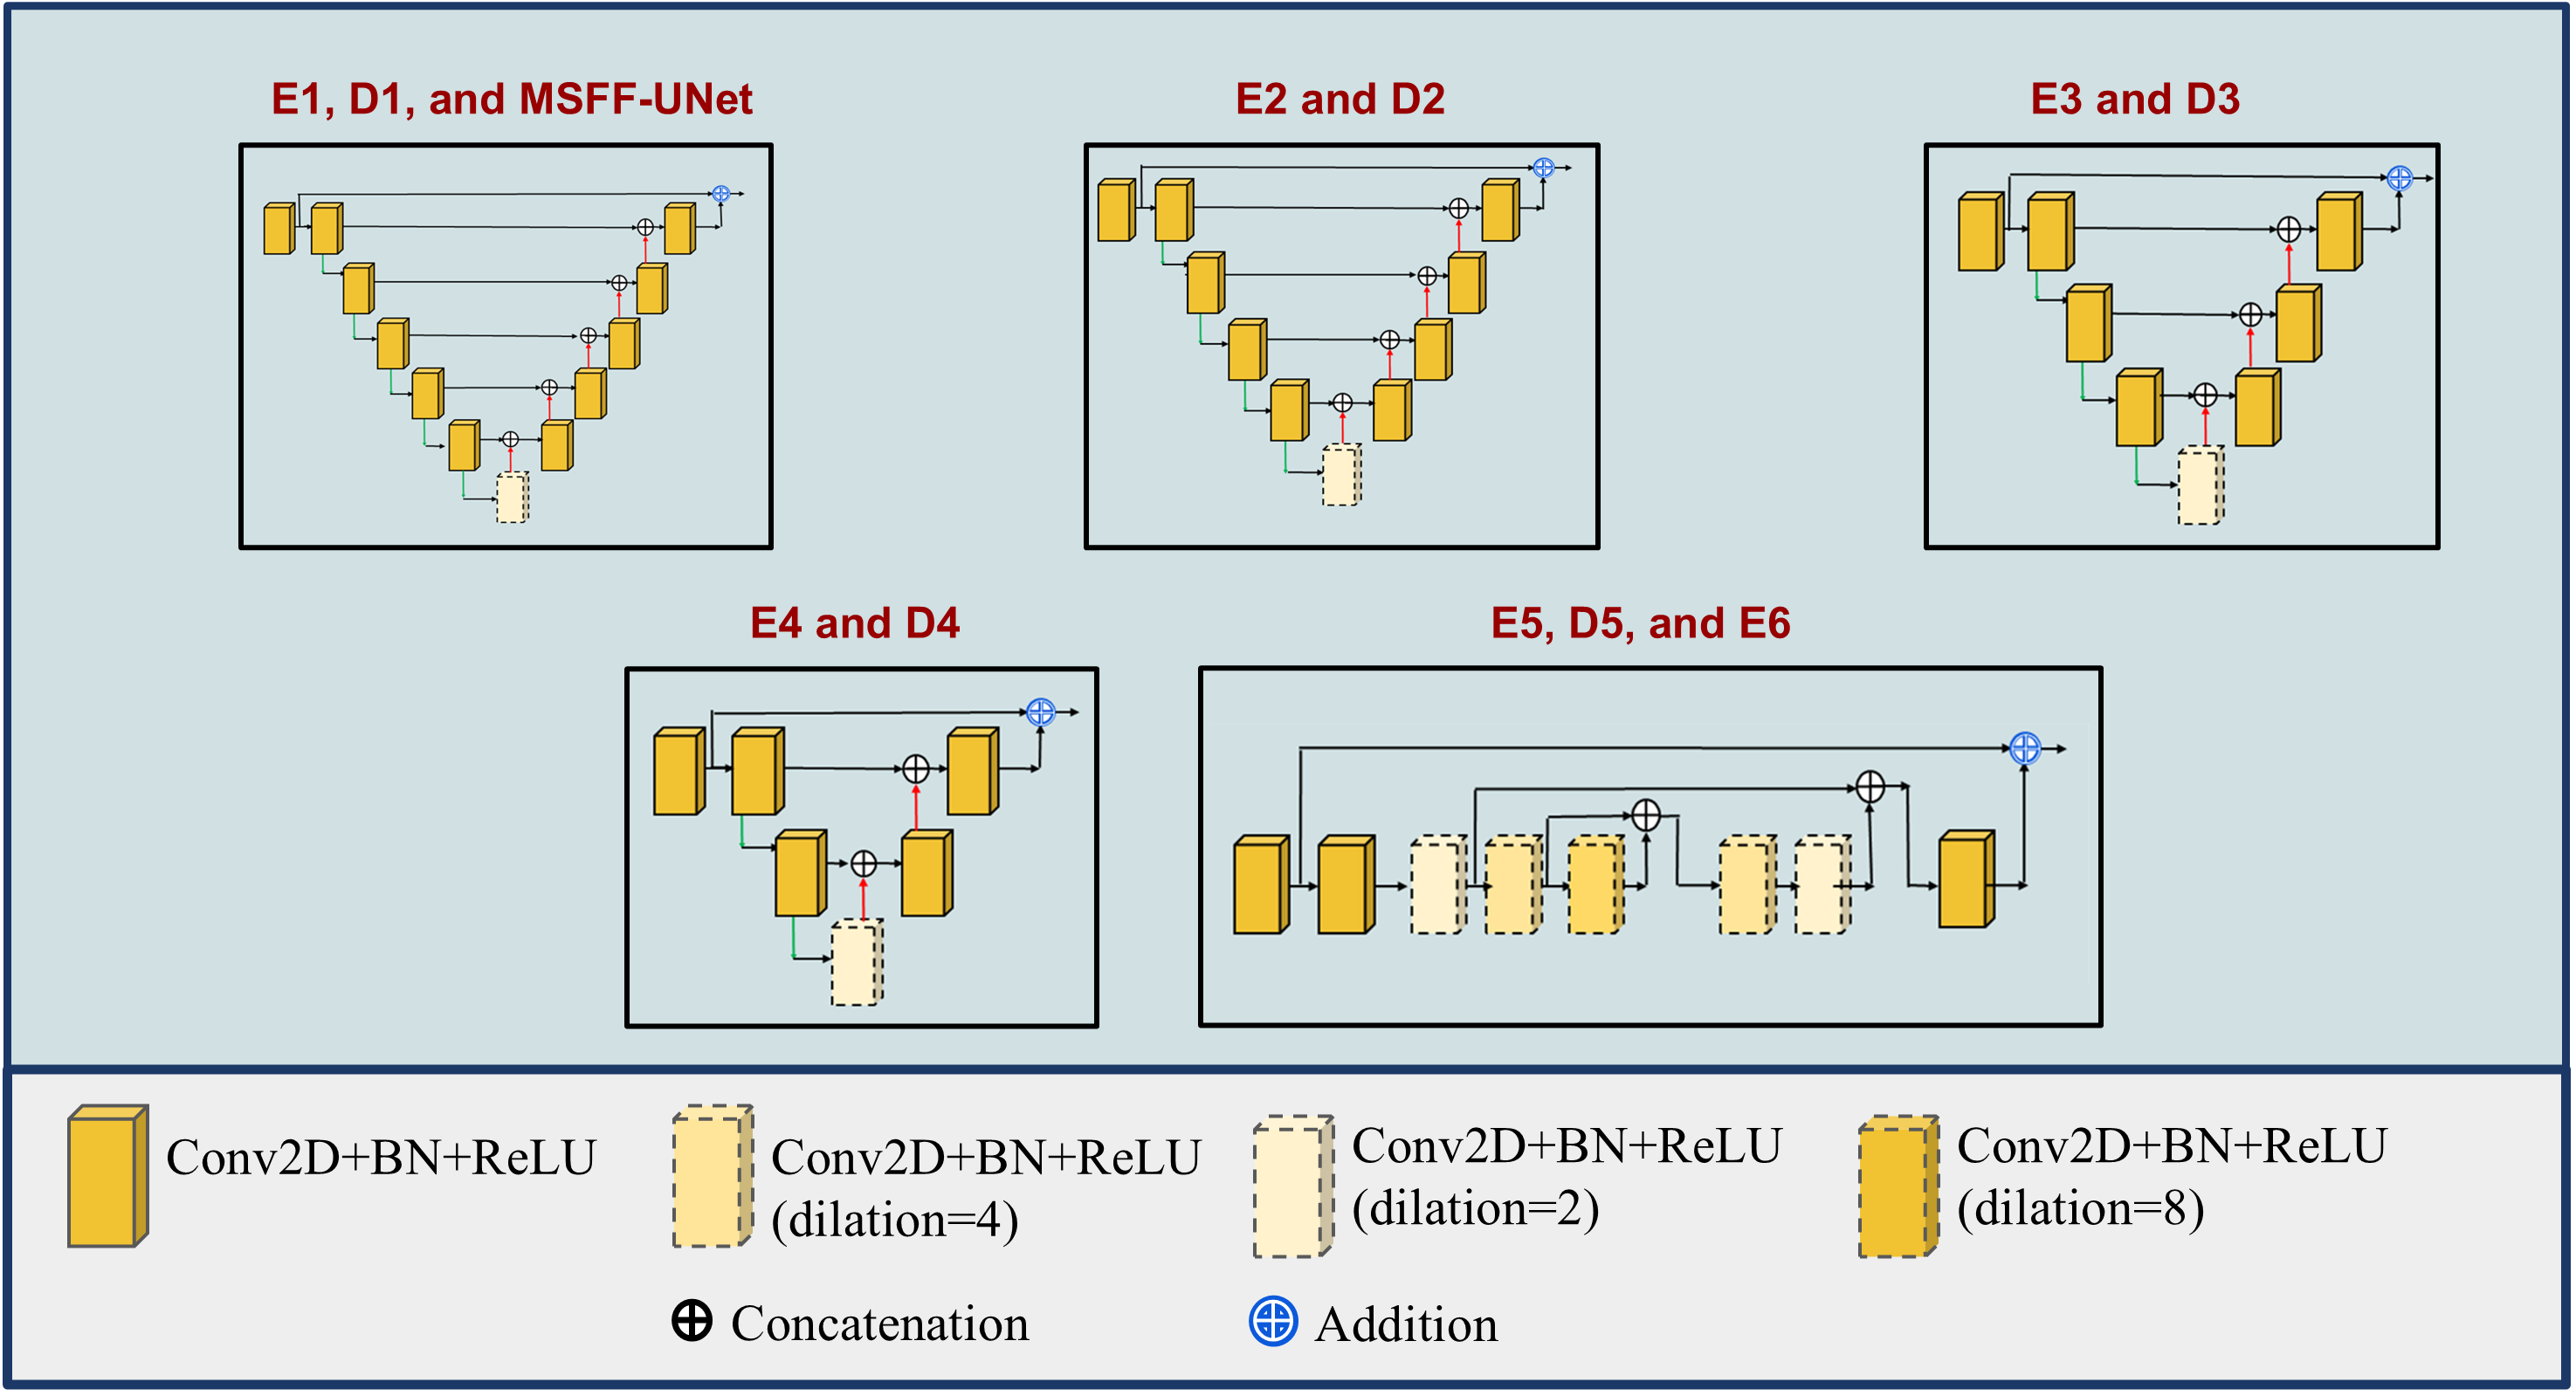
\includegraphics[width=\linewidth]{SFigure1.PNG}}
% \caption{Various UNet blocks utilized in both the main-network and sub-network.}

\caption{Detailed UNet block configurations used in MNSeg-Net. 
The blocks vary in depth depending on the stage of the encoder–decoder: (a) E1, D1, and MSFF-UNet employ the deepest structure; 
(b) E2/D2 and (c) E3/D3 progressively reduce depth; 
(d) E4/D4 adopt a shallow configuration; and 
(e) E5, D5, and E6 rely on dilated convolutions (dilation factors 2, 4, 8) to enlarge the receptive field without pooling or upsampling. 
This staged design balances representational power with computational efficiency.}

  \label{fig:all_UNet_models_config}
\end{figure*}






% \section{Patient-wise Equivalence Analysis of MNSeg-Net}

% A patient-wise Two One-Sided Tests (TOST) equivalence analysis was conducted to compare clinician-measured CSA with MNSeg-Net predictions. The analysis revealed variability across patients in terms of the equivalence outcomes. At the strict equivalence margin of $\pm 0.1$, none of the patients satisfied the equivalence criteria, suggesting that the differences between the predicted and clinician values exceeded this narrow threshold in all cases. When the margin was relaxed to $\pm 0.2$, only Patients 6 and 7 achieved equivalence, indicating partial consistency between model predictions and clinical measurements. At a wider margin of $\pm 0.5$, MNSeg-Net achieved equivalence for six patients (Patients 0, 1, 5, 6, 7, and 8), while four patients (Patients 2, 3, 4, and 9) continued to show meaningful differences from the clinician values.




% The results are presented in Table~\ref{tab:mnseg_equiv}, which reports the mean differences, 95\% confidence intervals, and equivalence outcomes for each patient across the evaluated margins. Collectively, these findings demonstrate the capability of MNSeg-Net to approximate clinician CSA measurements within clinically acceptable tolerance levels. For most patients, the model showed strong agreement with clinician-derived values, underscoring its potential for reliable clinical adoption. 





% \begin{table}[ht]
% \centering
% \caption{Patient-wise TOST Equivalence Results with 95\% Confidence Intervals (MNSeg-Net vs. Clinician CSA)}
% \begin{tabular}{|c|c|c|c|c|c|c|}
% \hline
% \textbf{Patient ID} & \textbf{Mean Diff} & \textbf{95\% CI Low} & \textbf{95\% CI High} & \textbf{±0.1} & \textbf{±0.2} & \textbf{±0.5} \\
% \hline
% 0 & -0.3599 & -0.5208 & -0.1989 & No& No& Yes \\
% 1 & -0.1929 & -0.3437 & -0.0421 & No& No& Yes \\
% 2 &  0.6124 &  0.3719 &  0.8529 & No& No& No\\
% 3 & -0.8487 & -1.1435 & -0.5538 & No& No& No\\
% 4 & -1.0546 & -1.2940 & -0.8152 & No& No& No\\
% 5 & -0.1358 & -0.2691 & -0.0026 & No& No& Yes \\
% 6 &  0.0111 & -0.1563 &  0.1785 & No& Yes   & Yes \\
% 7 &  0.0002 & -0.2205 &  0.2209 & No& Yes   & Yes \\
% 8 &  0.2327 &  0.0290 &  0.4363 & No& No& Yes \\
% 9 &  0.9284 &  0.7177 &  1.1391 & No& No& No\\
% \hline
% \end{tabular}
% \label{tab:mnseg_equiv}

% \end{table}



















\end{document}